\documentclass{article}

% Language setting
% Replace `english' with e.g. `spanish' to change the document language
\usepackage[english]{babel}
\usepackage[section]{placeins}
\usepackage{listings}
\usepackage{tabto}
% Set page size and margins
% Replace `letterpaper' with`a4paper' for UK/EU standard size
\usepackage[letterpaper,top=2cm,bottom=2cm,left=3cm,right=3cm,marginparwidth=1.75cm]{geometry}


% Useful packages
\usepackage{amsmath}
\usepackage{amssymb}
\usepackage{graphicx}
\usepackage[colorlinks=true, allcolors=blue]{hyperref}
\usepackage{float}
\usepackage[thinc]{esdiff}

\title{Assignment-2}
\author{S.Vishal CH18B020}

\begin{document}
\maketitle
\section*{Question-1}
Setting derivatives to zero,
\begin{align*}
    y + y^2 = 0 \implies y(y+1) = 0 \\
    \implies y = 0, -1
\end{align*}
\begin{align*}
    - x + \frac{1}{5}y - xy + \frac{6}{5}y^2 &= 0 \\
\end{align*}
If y = 0,
\begin{align*}
    - x + 0 - 0 + 0 &= 0 \\
    \implies x &= 0
\end{align*}
If y = -1, \\
$- x - \frac{1}{5} + x - \frac{6}{5} = 0$ \\
$\implies$ no solution. \\
Therefore only equilibrium point is (0,0). \\
\begin{align*}
    y + y^2 = 0 \implies y(y+1) = 0 \\
    \implies y = 0, -1
\end{align*}
Linearisation expression, 
\begin{align}
    \dot{x} = \begin{bmatrix}
\frac{\partial f1}{\partial x1} & \frac{\partial f1}{\partial x2}\\\\
\frac{\partial f2}{\partial x1} & \frac{\partial f2}{\partial x2} 
\end{bmatrix} \Tilde{x} + \begin{bmatrix}\frac{\partial f1}{\partial u1} & \frac{\partial f1}{\partial u2}\\\\
\frac{\partial f2}{\partial u1} & \frac{\partial f2}{\partial u2} \end{bmatrix}\Tilde{u}
\label{lineqn}
\end{align} 
where $\Tilde{x} = x - x^{*}$ and $\Tilde{u} = u - u^{*}$ and $x^{*}$ and $u^{*}$ is the point around which we are linearising. (an equilibrium/steady state). The derivatives are evaluated at the point around which we are linearising.
\[A = \begin{bmatrix}
0 & 1 + 2y\\\\
-1 - y & \frac{1}{5} + \frac{12}{5}y^2 - x
\end{bmatrix} \\
= \begin{bmatrix}
0 & 1\\
-1 & \frac{1}{5}
\end{bmatrix} \]
\begin{align*}
    \dot{x} &= \Tilde{y} \\
    \dot{y} &= - \Tilde{x} + \frac{1}{5}\Tilde{y}
\end{align*}
\section*{Question-2}
Setting $\dot{r} = 0$,
\begin{align}
    r(1-r^2) &= 0 \\
    \implies r &= 0, 1 \\
    1 - cos(\theta) &= 0 \\
    \implies \theta &= 2n\pi \quad n \in Z
\end{align}
(note that r can't be negative.) \\
we get the jacobian (matrix A) as,
$\begin{bmatrix}
1-3r^2 & 0\\
0 & sin(\theta)
\end{bmatrix}$
\subsection*{r = 0, $\theta = 2n\pi$}
Linearising around r = 0,
$A = \begin{bmatrix} 1 & 0 \\ 0 & 0\end{bmatrix} $
\begin{align*}
    \dot{r} &= \Tilde{r} \\
    \dot{\theta} &= 0
\end{align*}
\subsection*{r = 1, $\theta = 2n\pi$}
Linearising around r = 1,
$A = \begin{bmatrix} -2 & 0 \\ 0 & 0\end{bmatrix} $
\begin{align*}
    \dot{r} &= -2\Tilde{r} \\
    \dot{\theta} &= 0
\end{align*}
where, $\Tilde{r} = r-r^*$


\section*{Question-3}
Setting derivatives to 0,
\begin{align*}
    \sin(y) &= 0 \\
    \implies y &= \pm n\pi
    x - x^3 &= 0 \\
    \implies x &= -1, 0, 1
\end{align*}
To explain the behaviour around equilibrium points we need to find the eigen values of A matrix. \\ \\

$A = \begin{bmatrix} 0 & cos(y) \\ 1-3x^2 & 0\end{bmatrix} $ \\
\\
Finding eigen values,
\begin{align*}
    \begin{vmatrix} 0-\lambda & cos(y) \\ 1-3x^2 & 0-\lambda\end{vmatrix} &= 0 \\
    \implies \lambda^2 = (1 - 3x^2)cos(y)
\end{align*}
\begin{align}
    \begin{array}{|c|c|c|}
    \hline
    x,y    & y = 2n\pi  & y = (2n+1)\pi   \\
    \hline
    x = 0  & \lambda^2 >0 \implies \lambda = \pm c \therefore Saddle & \lambda^2 < 0 \implies \lambda = \pm j \therefore  center focus \\
    x = 1  & \lambda^2 < 0 \implies \lambda = \pm j \therefore  center focus & \lambda^2 >0 \implies \lambda = \pm c \therefore Saddle        \\
    x = -1 & \lambda^2 < 0 \implies \lambda = \pm j \therefore  center focus  & \lambda^2 >0 \implies \lambda = \pm c \therefore Saddle  
    \end{array}
\end{align}

\section*{Question-4}
Note that $x  + y + z = 1$ (since they are fractions). So instead of using 3 dependent states, we can reduce the system to just 2 states.
\begin{align}
    \dot{x} &= rx(1-x-y) \\
    \dot{y} &= ry(1-x-y) \\
\end{align}
Origin is an equilibrium point, and $x+y=1$ is a equilibrium subspace. The Jacobian is,
\begin{equation}
    \begin{bmatrix} r(1-2x-y) & -rx \\ -ry & r(1-x-2y) \end{bmatrix}
\end{equation}
\subsection*{At origin}
\begin{equation}
    \begin{bmatrix} r & 0 \\ 0 & r \end{bmatrix}
\end{equation}
Eigen values, $\lambda = r,r$. So origin is a stable equilibrium if $r<0$ which means x=y=0. Therefore, the situation where everyone is a centrist is the stable equilibrium in this case. And if a small number of people become rightist or leftist, they are brought back to being centrist. \\
On the other hand if $r>0$, the equilibrium is unstable. So if some people become rightist or leftist, the number of centrists starts reducing (moving away from equilibrium). And if $r=0$ obviously, there is no dynamics.\\
\subsection*{Subspace x + y = 1}
Parameterise the points as $\alpha$, $1-\alpha$.
\begin{equation}
    \begin{bmatrix} -r\alpha & -r\alpha \\ -r(1-\alpha) & -r(1-\alpha) \end{bmatrix}
\end{equation}
Eigen values of the matrix are $\lambda = 0, -r$.
If $r>0$ (hence, $\lambda<0$) all the trajectories converge to the equilibrium space. If $r<0$ (hence, $\lambda>0$) diverge from the equilibrium space. This means for $r>0$, the population evolves such that centrists population becomes 0 ($\because z = 1 - x - y = 0$). On the other hand, if $r<0$, small perturbation from the equilibrium space causes continous evolution away from it (resulting in everyone becoming centrists as deduced by observing stability of the equilibrium at origin).


\section*{Question-5}
Let 
\begin{align*}
    x &= \begin{bmatrix}r \\ \dot{r} \\ \theta \\ \dot{\theta} \end{bmatrix} 
    u = \begin{bmatrix}u_1 \\ u_2    \end{bmatrix} \\
\end{align*}
So the equations governing the dynamics are,
\begin{align}
    \dot{x_1} &= x_2 \\
    \dot{x_2} &= x_1x_4^2 - \frac{\beta}{x_1^2} + u_1 \\
    \dot{x_3} &= x_4 \\
    \dot{x_4} &= \frac{-2x_2x_4}{x_1} + \frac{u_2}{x_1}
\end{align}
Computing the Jacobian (from eqn \ref{lineqn}), \\
\begin{equation}
    A = \begin{bmatrix}  
    0 & 1 & 0 &  0 \\  \\
    \omega_0^2 + \frac{2\beta}{r_0^2} & 0 & 0 & 2r_0\omega_0\\  \\
    0 & 0 & 0 & 1\\ \\
    0 & \frac{-2\omega_0}{r_0} & 0 & 0
    \end{bmatrix}
\end{equation}
where $\omega_0 = \sqrt{\frac{\beta}{r_0^3}}$
\begin{equation}
    B = \begin{bmatrix}  
    0 & 0 \\
    1 & 0\\ 
    0 & 0\\
    0 & \frac{1}{r_0}
    \end{bmatrix}
\end{equation}
The equations governing the linearized system are,
\begin{align}
    \dot{x} &= A\Tilde{x} + B\Tilde{u} \\
    x &= \begin{bmatrix}r \\ \dot{r} \\ \theta \\ \dot{\theta} \end{bmatrix} 
    u = \begin{bmatrix}u_1 \\ u_2    \end{bmatrix} \\
    \Tilde{x} &= x - x^* \quad \quad \Tilde{u} = u - u^* \\
    \textrm{where } x^* &= \begin{bmatrix}r_0 \\ 0 \\ \omega_0t + \theta_0 \\
    \dot{\theta} \end{bmatrix}  \\
    \textrm{and, } u^* &= \begin{bmatrix}0 \\ 0    \end{bmatrix} 
\end{align}


\section*{Question-6}
Only equilibrium point is origin. Jacobian at equilibrium point is found to be,
\begin{align*}
    \begin{bmatrix} sin(1)  & 1 \\ -1 & sin(1)\end{bmatrix}
\end{align*}
% Eigen values are $\lambda = sin(1) \pm j$. Since $sin(1) > 0$, the equilibrium point is an unstable focus.
% Consider,
% \begin{align}
%     V(x) = x_1^2 + x_2^2 &= c. \\
%     \overline{\nabla}V &= 2x_1\hat{i} + 2x_2\hat{j}
% \end{align}
% Now we find a c such that
% \begin{align*}
%     \overline{\nabla}V.f(x) \leq 0 \\
%     \implies x(y + (x^3 + xy^2 - x)sin(\frac{1}{x^2+y^2-1})) + y(-x + (x^2y + y^3 - y)sin(\frac{1}{x^2+y^2-1}))) \leq 0 \\
%     \implies sin(\frac{1}{x^2+y^2-1}) (x^4 + 2x^2y^2 + y^4 + y^4 - x^2 - y^2) &\leq 0 \\
%     \implies sin(\frac{1}{x^2+y^2-1})((x^2 + y^2)^2 - (x^2 + y^2)) &\leq 0 \\
%     \implies ((x^2 + y^2)^2 - (x^2 + y^2)) &\leq 0 \quad (\because sin(\theta) \leq 1)
% \end{align*}
% This holds true when $x^2 + y^2 \leq 1$ $(\because a^2 \leq |a|$ if $|a| < 1) \implies c \leq 1$. So, trajectories starting in $M = {x^2 + y^2 \leq c}$ (where c follows the above condition) stays inside it. Therefore, by Poincare-Benedixson criterion a stable orbit exists.
Let's convert the equations to polar form.
\begin{align*}
    r &= \sqrt{x^2 + y^2} \\
    \dot{r} &= \frac{x\dot{x}}{\sqrt{x^2 + y^2}} + \frac{y\dot{y}}{\sqrt{x^2 + y^2}} \\
    &= (x^2 + y^2)(x^2 + y^2 - 1)sin(\frac{1}{x^2+y^2-1})\frac{1}{r} \\
    &= \frac{(r^2)(r^2-1)sin(\frac{1}{r^2-1})}{r} \\
\end{align*}
\begin{equation}
    \implies \dot{r} = \frac{(r^2)(r^2-1)sin(\frac{1}{r^2-1})}{r}
\end{equation}
\begin{align*}
    \dot{\theta} &= \frac{d}{dt}\tan^{-1}(\frac{y}{x}) \\ \\
    &= \frac{1}{1 + \frac{y^2}{x^2}}(\frac{\dot{y}}{x} - \frac{\dot{x}y}{x^2}) \\ \\
    &= \frac{x^2}{r^2}(\frac{-r^2}{x^2}) \\
    \implies \dot{\theta} &= -1
\end{align*}
We see $\dot{r} = 0$ has infinite solutions because of the sine term, and $\dot{\theta}$ is always a constant. So there are infinitely many limit cycles (i.e., where $\dot{r} = 0$ and $\dot{\theta}$ is a constant).


\section*{Question-7}
\subsection*{a)}
Jacobian yields,
\begin{align*}
    \begin{bmatrix} -1 & 0\\ 0 & -1 \end{bmatrix} \\
    \lambda  = -1, -1
\end{align*}
(The derivative of the log term goes to zero in the limit).  \\
So the origin is a stable node.
\\
\subsection*{b)}
\begin{figure}[h!]
\centering
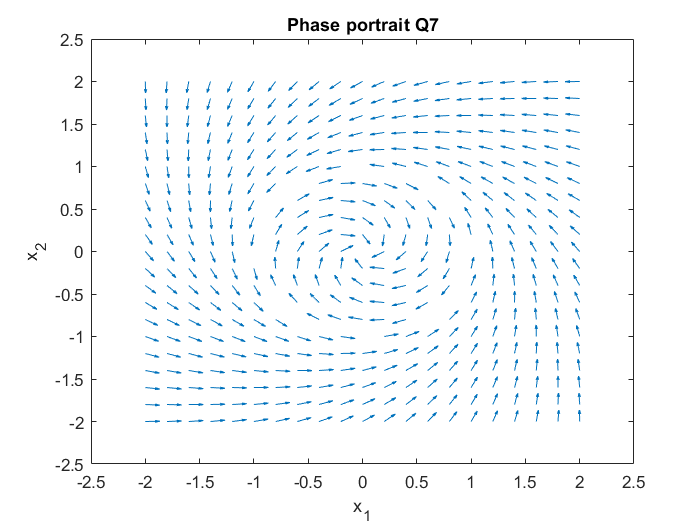
\includegraphics[width=0.8\textwidth]{plots/Q7b.png}
\caption{\label{7b}Phase Portrait Q7b}
\end{figure}
\FloatBarrier
From the figure, we can see that trajectories close to origin spiral towards it, showing that it is a stable focus.
\\
\subsection*{c)}
Although the function is continously differentiable, at origin, the derivatives converge to the respective values only in the limit. So, the Taylor series expansion is likely to not converge. This means the function is not in the neighbourhood of $x_1, x_2 = (0,0)$. Since the function is not analytic, the linearization result differs from reality.

\section*{Question-8}
\subsection*{a)}
We can recast the system in state-space form (with $y$ and $\dot{y}$ as the respective states) as,
\begin{align*}
    \dot{x_1} = x_2
    \dot{x_2} = - x_1 - \epsilon(x_2)(1 - x_1^2 - x_2^2)
\end{align*}
Jacobian is,
\begin{align*}
    \begin{bmatrix} 0 & 1 \\ -1 & \epsilon \end{bmatrix}
    \implies \lambda = \epsilon \pm j
\end{align*}
The equilibrium is unstable for $\epsilon > 0$. Consider,
\begin{align}
    V(x) = x_1^2 + x_2^2 &= c. \\
    \overline{\nabla}V &= 2x_1\hat{i} + 2x_2\hat{j}
\end{align}
Now we find a c such that
\begin{align*}
    \overline{\nabla}V.f(x) &\leq 0 \\
    \implies 2x_1x_2 + 2x_2(-x_1 + \epsilon(1-x_1^2-x_2^2)) &\leq 0 \\
    \implies \epsilon(1 - x_1^2 - x_2^2) &\leq 0 \\
    \forall \epsilon > 0, \\
    x_1^2 + x_2^2 \leq 1
    \implies c \leq 1
\end{align*}
So, trajectories starting in $M = {x_1^2 + x_2^2 \leq c}$ (where c follows the above condition) stays inside it. Therefore, by Poincare-Benedixson criterion a stable orbit exists.

\subsection*{b)}
Jacobian is,
\begin{align*}
    \begin{bmatrix} 0 & 1 \\ -1 & 2 \end{bmatrix}
    \implies \lambda = 1, 1
\end{align*}
So, the equilibrium is unstable. Consider,
\begin{align}
    V(x) = x_1^2 + x_2^2 &= c. \\
    \overline{\nabla}V &= 2x_1\hat{i} + 2x_2\hat{j} \\
\end{align}
Now we find a c such that
\begin{align*}
    \overline{\nabla}V.f(x) &\leq 0 \\
    \implies x_1x_2 - x_1x_2 + 2x_2^2(2 - 3x_1^2 - 2x_2^2) \leq 0 \\
    \implies (3x_1^2 + 2x_2^2) \geq 2\\
    \impliedby 2x_1^2 + 2x_2^2 \geq 2 \\
    \implies c \geq 1
\end{align*}
So, trajectories starting in $M = {x_1^2 + x_2^2 \leq c}$ (where c follows the above condition) stays inside it. Therefore, by Poincare-Benedixson criterion a stable orbit exists.

\subsection*{c)}
Jacobian is,
\begin{align*}
    \begin{bmatrix} 0 & 1 \\ -1 & 1 \end{bmatrix}
    \implies \lambda = \frac{1 \pm \sqrt{3}j}{2}
\end{align*}
The equilibrium is unstable for $\epsilon > 0$. Consider,
\begin{align}
    V(x) = 3x_1^2 + 2x_1x_2 + 2x_2^2 &= c. \\
    \overline{\nabla}V &= (6x_1 + 2x_2)\hat{i} + (2x_1 + 4x_2)\hat{j}
\end{align}
Now we find a c such that
\begin{align*}
    \overline{\nabla}V.f(x) &\leq 0 \\
    \implies (6x_1 + 2x_2)x_2 + (2x_1 + 4x_2)(-x_1 + x_2 - 2(x_1 + 2x_2)x_2^2 &\leq 0 \\
    \implies 6x_1x_2 + 2x_2^2 - 2x_1^2 + 2x_1x_2 - 4x_1x_2 + 4x_2^2 - 4(x_1 + 2x_2)^2x_2^2 &\leq 0 \\
    \implies - 2x_1^2 + 4x_1x_2 + 6x_2^2 - 4(x_1 + 2x_2)^2x_2^2 &\leq 0 \\
    \implies -2(x_1^2 + x_2^2) + 4x_2(x_1 + 2x_2) - 4(x_1 + 2x_2)^2x_2^2 &\leq 0 \\
    \implies -2(x_1^2 + x_2^2) + 1 - (1 - 2x_2(x_1 + 2x_2))^2 &\leq 0 \\
    -2(x_1^2 + x_2^2) + 1 - (1 - 2x_2(x_1 + 2x_2))^2 &\leq -2(x_1^2 + x_2^2) + 1 \leq 0 \\
    \implies x_1^2 + x_2^2 &\geq -\frac{1}{2}
\end{align*}
So, trajectories starting in $M = {3x_1^2 + 2x_1x_2 + 2x_2^2 \leq c}$, where c is such that the surface $V(x) = c$ contains the circle $x_1^2 + x_2^2 = \frac{1}{2}$ in its interior, stays inside it. Therefore, by Poincare-Benedixson criterion a stable orbit exists.



\section*{Question-9}
Equilibrium point is origin. \\
Using the fact that $\diff{}{x}tanh(x) = sech^2(x)$, and $tanh(0) = 0$, the Jacobian is found to be, \\
\begin{align*}
    \begin{bmatrix}  \frac{-1}{\tau} + \lambda & -\lambda \\\\ \lambda & \frac{-1}{\tau} + \lambda \end{bmatrix}
\end{align*}
Eigen values were found to be, $\lambda = - \frac{1}{\tau} \pm j$. The real part is greater than zero as long as $\lambda\tau > 1$. Therefore, the equilibrium is unstable.
Consider,
\begin{align}
    V(x) = x_1^2 + x_2^2 &= c. \\
    \overline{\nabla}V &= 2x_1\hat{i} + 2x_2\hat{j}
\end{align}
Now we find a c such that
\begin{align*}
    \overline{\nabla}V.f(x) &\leq 0 \\
    \implies 2x_1(\frac{-x_1}{\tau} + tanh({\lambda}x_1) - tanh({\lambda}x_2)) + 2x_2(\frac{-x_2}{\tau} + tanh({\lambda}x_1) + tanh({\lambda}x_2)) &\leq 0 \\
    \implies -x_1^2 - x_2^2 + x_1tanh({\lambda}x_1) - x_1tanh({\lambda}x_2) + x_2tanh({\lambda}x_1) + x_2tanh({\lambda}x_2) &\leq 0
\end{align*}
Substituting $|tanh(x)| = 1$, $x_1 = rcos(\theta) \leq r$, and $x_2 = rsin(\theta) \leq r$ ,
\begin{align*}
    -\frac{r^2}{\tau} + r + r + r + r &\leq 0 \\
    \implies r &> 4\tau \implies c > 16\tau^2
\end{align*}
So trajectories starting in $M = {r \leq c}$ (where c follows the above condition) stays inside it. Therefore, by Poincare-Benedixson criterion a stable orbit exists.


\section*{MATLAB code for q7}
\subsection*{Contents}

\begin{itemize}
\setlength{\itemsep}{-1ex}
   \item derivatives
   \item Phase portrait
   \item function to evaluate derivatives in a mesh
\end{itemize}
\begin{verbatim}
clear; close all;
\end{verbatim}


\subsection*{derivatives}

\begin{verbatim}
f1 = @(x1,x2)(-x1 - x2/log(sqrt(x1^2+x2^2)));
f2 = @(x1,x2)(-x2 + x1/log(sqrt(x1^2+x2^2)));
\end{verbatim}


\subsection*{Phase portrait}

\begin{verbatim}
lim = 2; N = 21;
[X,Y,U,V] = derivatives(lim,N,f1,f2);
% Use quiver to plot; S = 0.75 to ensure arrows don't intersect
figure;
quiver(X,Y,U,V,0.5);
xlabel('x_1'); ylabel('x_2');
title('Phase portrait Q7');
\end{verbatim}


\subsection*{function to evaluate derivatives in a mesh}

\begin{verbatim}
function [X,Y,U,V] = derivatives(lim,N,f1,f2)
    % ---------------------------------------------------------------------
    % function to generate derivatives
    % lim - limits of the x,y grid of the plot. derivatives will be
    % evaluated at points between -lim to +lim
    %
    % N - number of points on each axis
    %
    % f1 - x derivative (xdot)
    % f2 - y derivative (ydot)
    % ---------------------------------------------------------------------
    % Generate mesh
    x = linspace(-lim,lim,N);
    y = linspace(-lim,lim,N);
    [X,Y] = meshgrid(x,y);
    % Variables to store derivatives
    U = zeros(size(X));
    V = zeros(size(X));
    for i = 1:length(X)
        for j = 1:length(Y)
            % Evaluate the derivatives
            u = f1(X(i,j),Y(i,j));
            v = f2(X(i,j),Y(i,j));
            r = sqrt(u^2+v^2);
            % Normalizing them to 1 and storing
            U(i,j) = u/r;
            V(i,j) = v/r;
        end
    end
end
\end{verbatim}

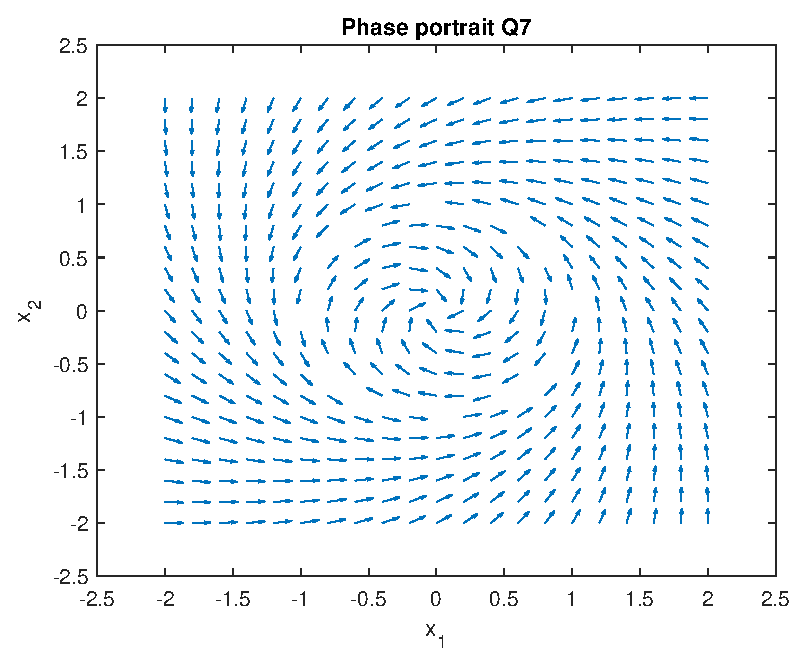
\includegraphics [width=4in]{Q7_01.eps}
\section*{References}
\begin{itemize}
    \item Students discussed with:
    \begin{enumerate}
        \item Karthik S ME18B149
    \end{enumerate}
    \item Course notes used:
    \begin{enumerate}
        \item Class notes
    \end{enumerate}
    \item Hassan Khalil
\end{itemize}
\end{document}